%including quality management and risk management (with a mandatory joint
%governing structure for EID and EJD projects)


%Required sub-headings:
\subsubsection{Network organization and management structure}
\label{sub:networkOrganization}
%including financial management strategy, strategy for dealing with scientific misconduct

%This table seems not needed...
%\begin{wraptable}{r}{0.36\textwidth}
%\vspace{-5mm}
%\small
%\caption{\small WP coordinators\label{tab:WPC}}
%\begin{center}
%\begin{tabular}{cl}
%\toprule
%WP1 & Caterina Doglioni \\
%WP2 & Anna Sfyrla \\
%WP3 & Vladimir Gligorov \\
%WP4 & Lionel Lacassagne \\
%WP5 & Johannes Albrecht (LHCb), Peter Christiansen (ALICE), Monica Dunford (ATLAS), Mikko Voutilainen (CMS)\\
%WP6 & Pavel Starovoitov, Nicolas Meric \\
%WP7 & Brian Petersen \\
%\bottomrule
%\end{tabular}
%\end{center}
%\vspace{-5mm}
%\end{wraptable} 
WP1 is dedicated to the management of \acronym. As specified in the WP description, the Project Coordinator (PC) will be Doglioni from \lundentity. 
She will benefit from the experience gained coordinating working groups in her collaboration, in the LHC-wide LHC Physics Center, as HEP Software Foundation convenor, as well as from her education that connected academia and industry.
The PC will act as the bridge between the Network and the EU and will be in charge of the management structure of \acronym, as well as of keeping an up-to-date overview of the network progress for the governing bodies of the network using the OmniPlan software and creating the infrastructure for network-wide communication as described in Sec.~\ref{sec:CommPub}. 
The PC will also drive the signature of the \textbf{Grant Agreement} (GA) and \textbf{Consortium Agreement} (CA) between all the nodes. 
The process leading to this will define the final structure of the Network, the employment status of the ESRs, Intellectual Property Right aspects and training structure, and it
will be steered by the PC and by the Work Package coordinators presented in Sec.~\ref{sec:WPdescription}.%table ~\ref{tab:WP}.  
%\footnote{In the case of WP5 (Physics applications), there is one responsible per LHC experiment represented in \acronym}. 
The WP coordinators will be responsible for the overall coherence and deliverables of their respective WP, the management of risks concerning their WP, and the reports of the progress in the WP they coordinate through the PCDPs. 
All WP coordinators including the PC and the Project Manager hired to support the PC will form the \acronym management board and meet bi-monthly to discuss the network progress. 

Alongside the management board, the Network will have two main discussion and decision-making bodies: an Executive Board (EB) and the Supervisory Board (SB).
These are pictured in the following figures and described in detail in Sec.~\ref{sub:jointGoverningStructure}. 

%%\begin{figure}[!htpb]
%%	\vspace{-5mm}
%	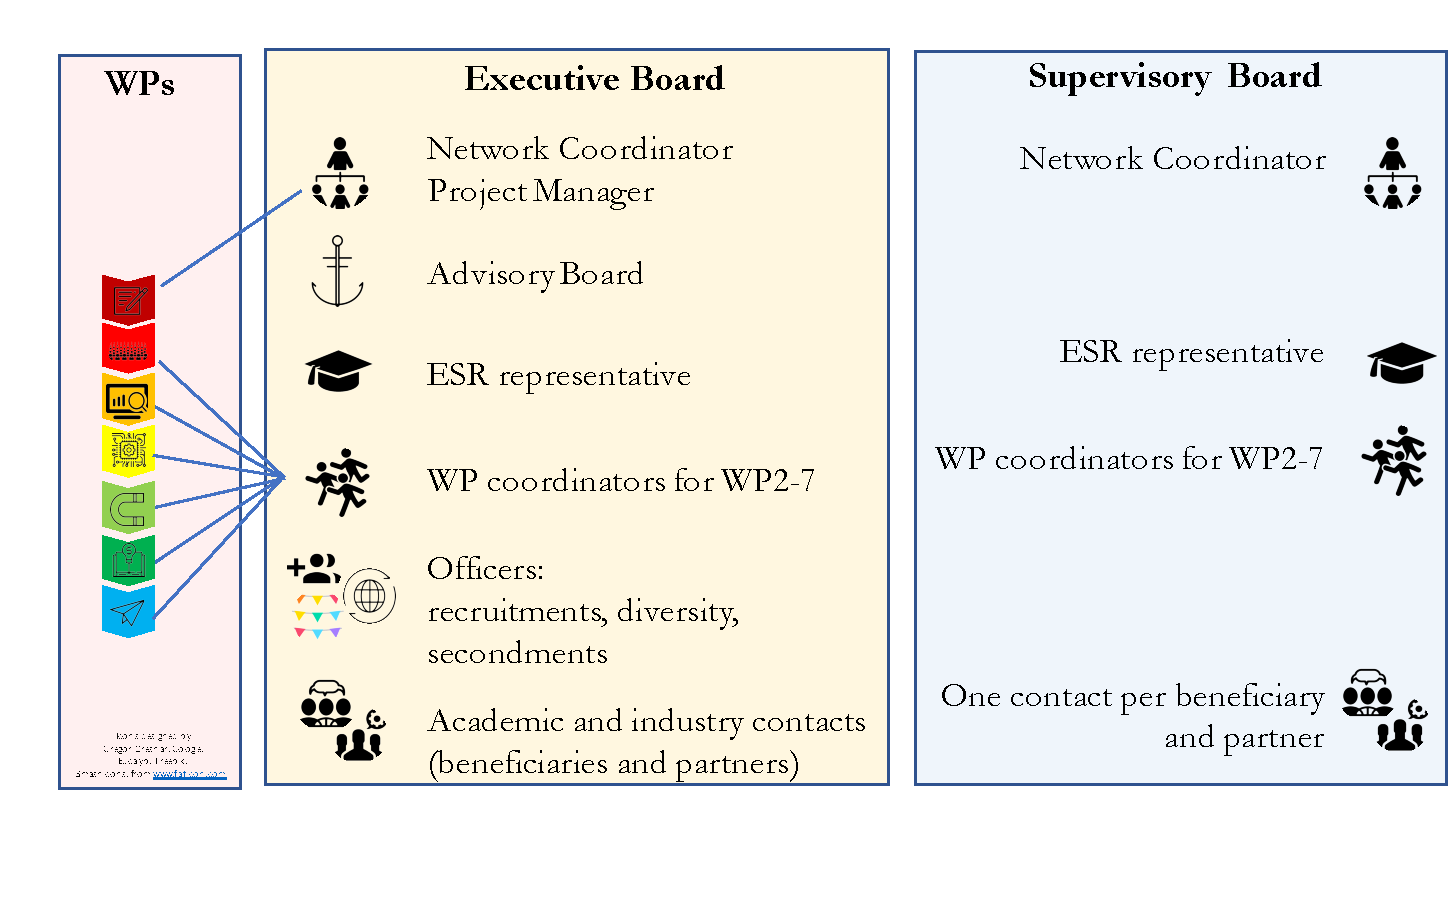
\includegraphics[width=0.7\textwidth]{figs/ManagementStructure.png} %scienceStructure_2.pdf}
%    \vspace{-5mm} 
%%	\caption{Management structure of \acronym.}
%	\label{fig:scienceStructure.pdf}
%%    \vspace{-2mm} 
%%\end{figure}

Official network communication, including decisions taken in EB and SC meetings, will be transmitted on the
existing network e-mail list \texttt{smarthep-participants@cern.ch}. The archives of this mailing list will be available, except in matters requiring non-disclosure. 
In those cases, communication will happen between %by phone and via e-mail involving 
the interested parties according to the regulations of each of the participants involved. 
A "virtual corridor" for the network has already been created at \cern using Mattermost software for rapid, non-official communication and collaboration,
allowing network members to create channels for discussion and effectively share documents, software, and announcements.
%Mattermost allows users to create channels for discussion of given topics through instant messaging, and is integrated with a number of other software package for effectively sharing documents, software and announcements.
%Mattermost effectively builds a virtual corridor in a software system. Mattermost promotes a flat hierarchy between the members of a team or a channel, but it also allows for channels that can only be joined by invitation. The typical use cases here are e.g. the communication among ESRs working on similar projects in geographically different locations, as well as the rapid discussion of network matters among the partners and beneficiaries.  The use of Mattermost to build a virtual corridor is an integral part of this proposal,
%and one that will strenghten collaboration across \acronym researchers for years to come. 

%CD: this is left for the figure
%\vspace{-4mm}
%\begin{wrapfigure}{l}{10cm}
%\begin{center}
%\includegraphics[width=0.75\textwidth]{figs/management2.pdf}
%\caption{\acronym management structure}
%\label{fig:management}
%\end{center}
%\vspace{-5mm}
%\end{wrapfigure}
%\vspace{-4mm}
%
\vspace{-2mm}
\subsubsection{Joint governing structure}% (mandatory for EID and EJD projects)}
\label{sub:jointGoverningStructure}

The EB is the extended project management body of \acronym. 
It is composed of the PC, coordinators of all WPs, a \textbf{student representative} elected from a board that the ESRs will be encouraged to form for their own discussion, three officers responsible for \textbf{recruitment, diversity and secondment} matters, and representatives from each \textbf{academic and industrial beneficiary and partner}. 
The EB is expected to meet via teleconference at least once every three months, as well as on demand.
It is a forum where all WP coordinators and contact persons report on their progress, results or other issues relevant for the Network. 
Action items arising from these reports might be: a communication strategy for a particular publication, the formation of a task force to deal with an identified risk or failure, a new avenue of research or a new product to be developed. 
These meetings will be chaired by the PC and minuted with listed action items. 
Draft minutes will be released shortly after the meeting, and final minutes within a week. 
Each EB meeting will follow up on outstanding action items.
The EB will meet physically during the first days of Network-wide events, and prepare the agenda for the SB meetings. 
The EB will also serve as a point of contact with all \acronym stakeholders, and provides support to the nodes organizing Network-wide events.
Finally, the EB will be able to propose changes to the plans presented in this proposal to the SB.

%CD: this is left for the figure
%\vspace{-4mm}
\begin{wrapfigure}{l}{1.1\textwidth}
%\begin{figure}[!htb]
\begin{center}
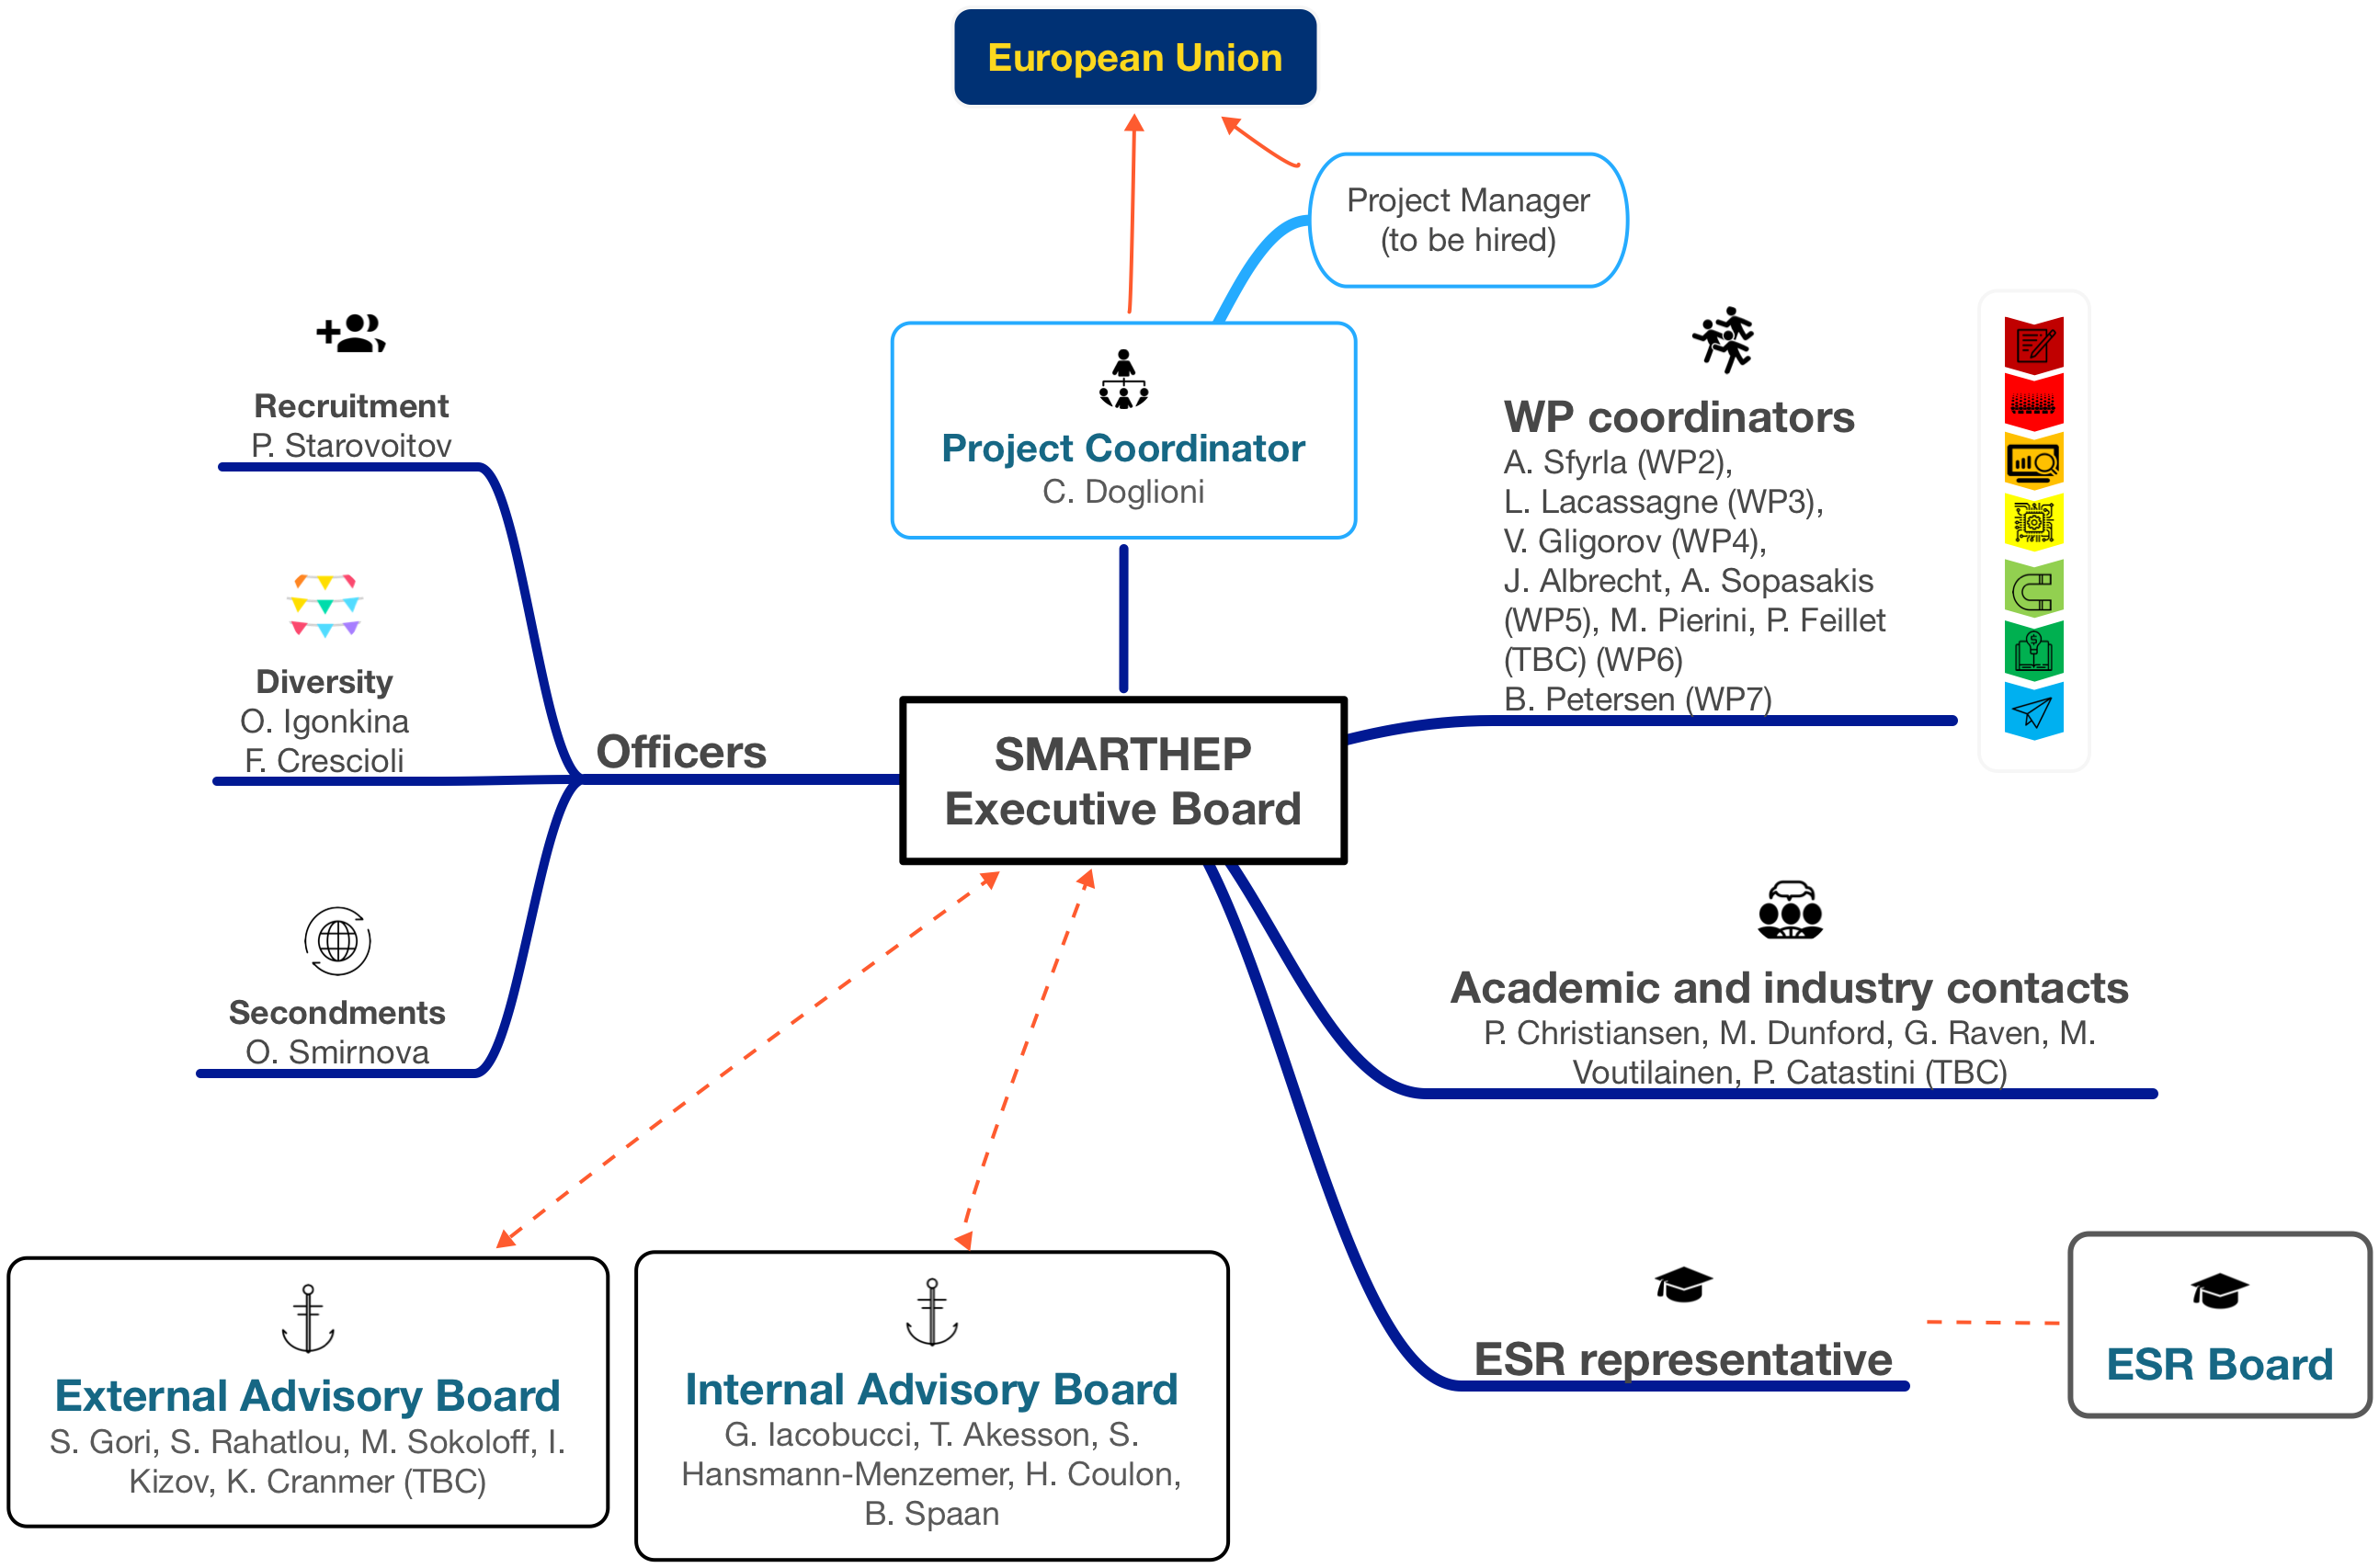
\includegraphics[width=\textwidth]{figs/SMARTHEP_Boards.png} %scienceStructure_2.pdf}
\caption{\acronym Executive Board (EB)}
\label{fig:management}
\end{center}
\vspace{-5mm}
%\end{figure}
\end{wrapfigure}
%\vspace{-4mm}


The EB will receive advice from the \textbf{Internal and External Advisory Boards}, two groups of senior physicists that will help consolidating the managerial experience of the junior researchers in the network. 
The Internal Advisory Board is composed of senior professors from the beneficiary institutes mentioned in Sec.~\ref{subsub:qual_supervisors}, who have extensive experience in project management and coordination. 
The External Advisory Board is composed of experienced professors that are not employed in beneficiary or partner institutes, who will also participate in the training events. 
It includes Prof. Stefania Gori from UCSC, an expert in theoretical physics phenomenology, Prof. Mike Sokoloff from U. Cincinnati, one of the founding member of the HEP Software Foundation, Prof. Ivan Kisel from FIAS, who is one of the pioneers of many reconstruction methods for particle tracks in high energy physics and Prof. Shahram Rahatlou from University of Rome Sapienza, who has been the CMS Physics Coordinator. %and Prof. Kyle Cranmer from NYU's center for Data Science, an expert in statistics, machine learning and data preservation. 
The members of this board will act as external observers to the network and offer advice on the impact and dissemination activities as seen from the broader community. 
They will also help resolve conflicts between participants that may arise within the network.
The External and Internal Advisory Board members will be invited to the \acronym yearly meetings. 

\vspace{-2mm}
\subsubsection{Supervisory board}

%\begin{wrapfigure}{l}{1.1\textwidth}
%%\begin{figure}[!htb]
%\begin{center}
%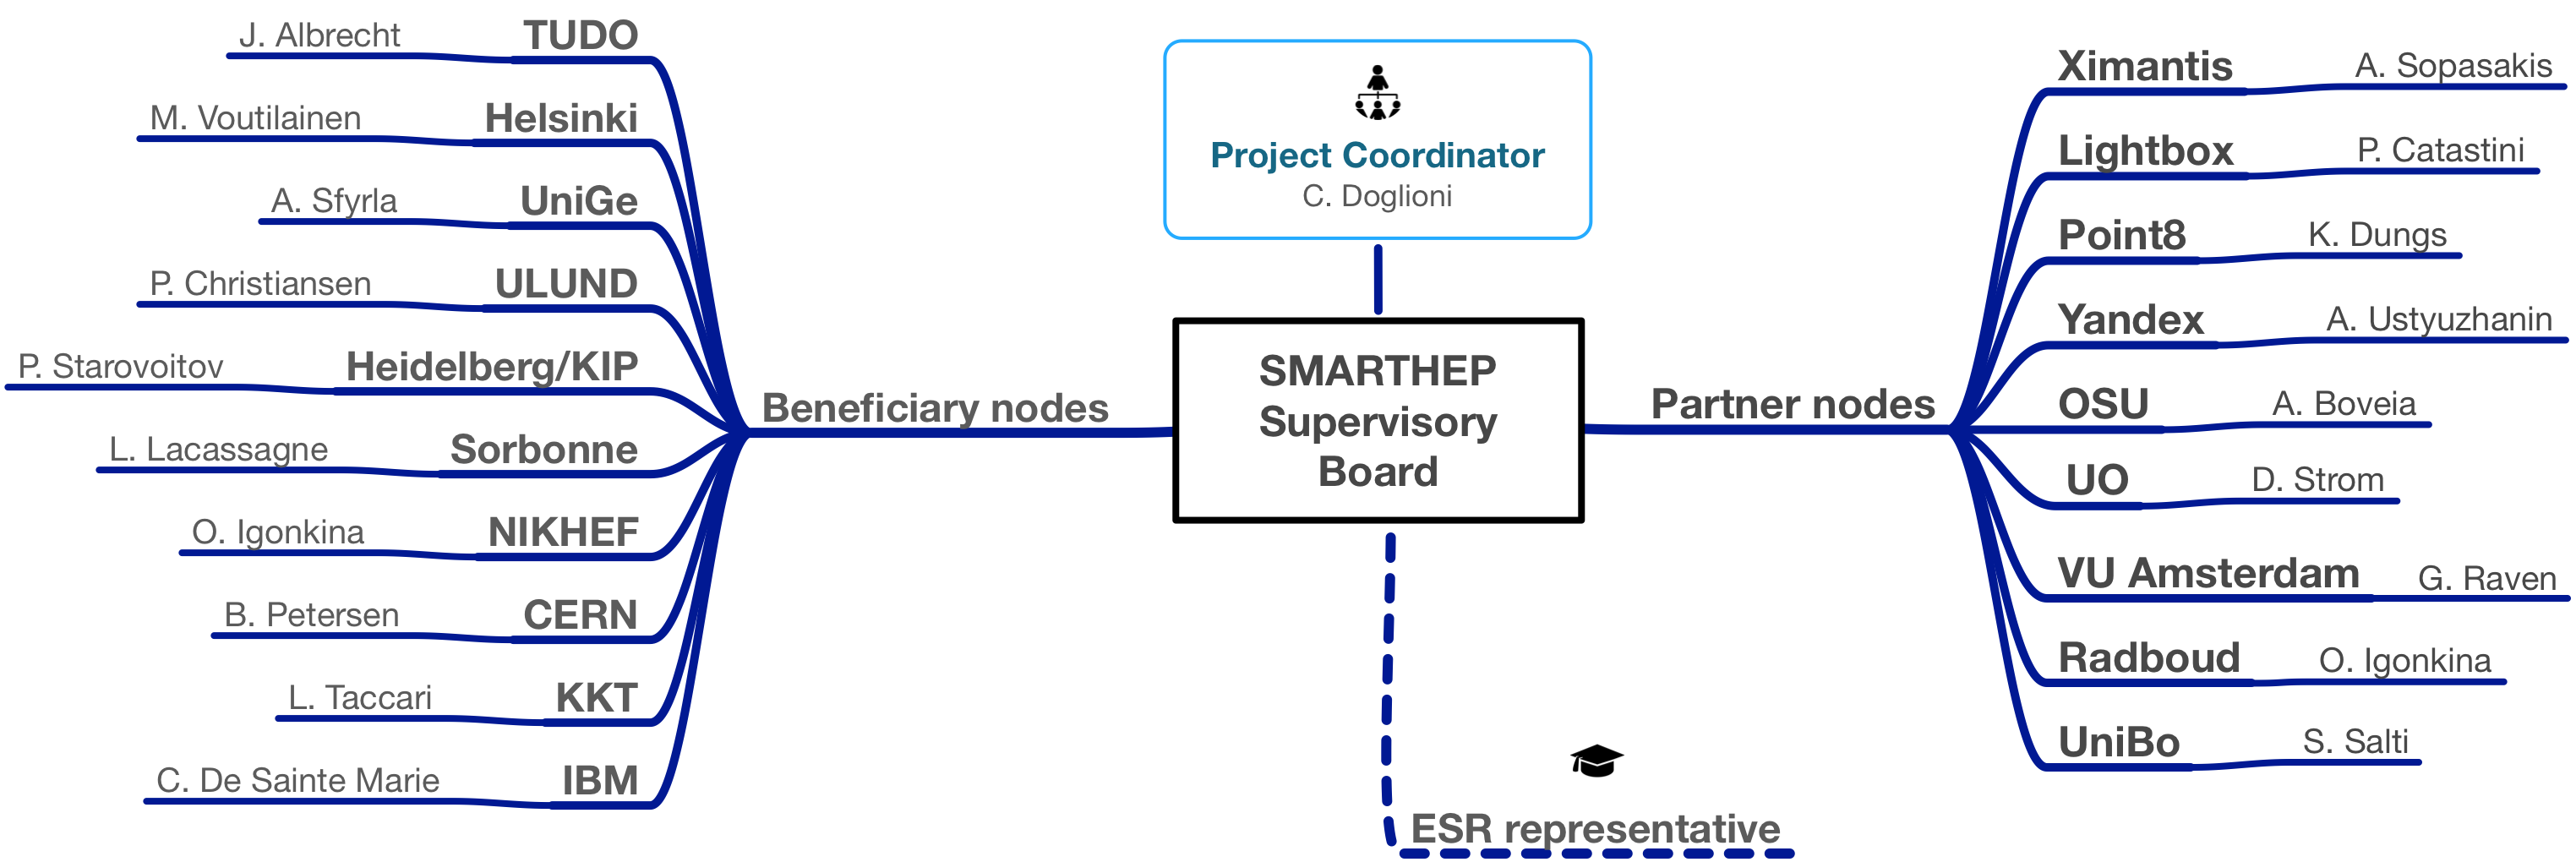
\includegraphics[width=\textwidth]{figs/SMARTHEP_SupervisoryBoard.png} %scienceStructure_2.pdf}
%\caption{\acronym Supervisory Board (SB)}
%\label{fig:management}
%\end{center}
%\vspace{-5mm}
%%\end{figure}
%\end{wrapfigure}
%%\vspace{-4mm}

The SB drafts the CA and is the decision-making body of \acronym in matter of training and project, by majority vote. 
It receives advice and action items from the EB. 
Each \acronym node has a single vote in the SB. They are usually represented through their main contact person as specified in the List of Beneficiaries and List of Partner Organizations Tables.
The student representative will be allowed to participate and vote in the SB, but the SB reserves the right to hold closed meetings in case of items that are critical for one or more ESR (e.g. failed progress, crisis management, scientific misconduct). 
The approval of the PCDPs will not include the ESR vote.
The work plan presented in this proposal will have to be approved by the SB at the Kick-off meeting, to be held during month 2 of the project. 
The SB will also have to approve any measurement proposed by the EB and the PCDP of all the ESRs.
The SB will monitor the progress of the Network, including the quality of training and supervision, and will monitor and take action on scientific misconduct as per the the The European Code of Conduct for Research Integrity\footnote{\url{https://ec.europa.eu/research/participants/data/ref/h2020/other/hi/h2020-ethics_code-of-conduct_en.pdf}}. 
Apart from the Kick-off meeting, the SB will meet yearly in the special Network-Wide events organised by \acronym. 
These meetings will be chaired by the PC.

\vspace{-2mm}
\subsubsection{Recruitment strategy}

%Recruitment
%The following sections of the European Code of Conduct for the Recruitment of Researchers refer specifically to recruitment and selection:
%Employers and/or funders should establish recruitment procedures which are open, efficient, transparent, supportive and internationally 
%comparable, as well as tailored to the type of positions advertised.
%Advertisements should give a broad description of knowledge and competencies required, and should not be so specialised as to discourage 
%suitable applicants. Employers should include a description of the working conditions and entitlements, including career development prospects. 
%Moreover, the time allowed between the advertisement of the vacancy or the call for applications and the deadline for reply should be realistic.
%Selection
%Selection committees should bring together diverse expertise and competences and should have an adequate gender balance and, where appropriate
%and feasible, include members from different sectors (academic and non-academic) and disciplines, including from other countries and with relevant
%experience to assess the candidate. Whenever possible, a wide range of selection practices should be used, such as external expert assessment and
%face-to-face interviews. Members of selection panels should be adequately trained.

\acronym will recruit in compliance with the ``European Code of Conduct for the Recruitment of Researchers''. 
\acronym is committed to appointing the ESRs in a gender unbiased way and candidates will be selected regardless of their race, religion, sexual orientation or disability. 
We are aware that marginalized groups are significantly underrepresented among job applicants and will take proactive steps to advertise \acronym ESR positions among them and highlight their inclusiveness, as discussed in a dedicated section (Sec.~\ref{sub:genderEO}).
\acronym will have a common job advertisement template and a dedicated information webinar for prospective ESRs at the kick-off meeting. Work on the recruitment will start in advance of the CA signature so that all ESRs are recruited by month 8.
Positions will be announced and described in detail on appropriate portals at the national, European, and international level, e.g.
on the Euraxess portal, our web page and social media.

Once recruitment for each node is completed, the corresponding beneficiary main contact will inform the recruitment officer and the relevant WP coordinator(s) and bring the proposal to the EB meeting for approval. 
As part of this approval, the two best-ranked runners-up will be reviewed by the recruitment and diversity officers, as EB members not involved in the original recruitment. 
The goal is to verify that the selection process was unbiased with respect to gender, race, religion, sexual orientation or disability. 
In particular, the review will establish whether there was any unconscious bias on the part of the recruiting panel. 
Starovoitov (\heidelbergshort) will serve as~\textbf{recruitment officer} with a seat in the EB overseeing the recruitment procedure. 

\vspace{-2mm}

\subsubsection{Progress monitoring and evaluation of individual projects}
\label{sub:progressMonitoring}
 
Several progress monitoring and evaluation plans are foreseen:
\begin{itemize}%[topsep=0pt,nosep]
\item A PCDP will be created for each ESR, and approved first by the supervisors and then by the WP coordinator and SB.
\item Supervisors will report on ESR progress to the WP coordinator where the ESR is working, as well as in EB and SB meetings. 
Supervisors will also communicate back the feedback coming from the ESR to the SB.  
\item Each secondment responsible (partner or beneficiary) will write a short progress report of the ESR's work and achievements at the end of the secondment, monitored by the dedicated \textbf{secondment officer} Smirnova (\lundentity). 
Secondments are the basis of lasting relationships between the ESR and the network partners maintained beyond \acronym. 
\item ESRs will present their work in talks and/or posters in the yearly network events, as well as in international conferences when major milestones are reached. 
The ESR presentations and posters will be collected by the \textbf{WP7 responsible} Petersen (\cernentity) on the \acronym website. 
\item Yearly appraisal meetings will be held by beneficiaries, and chaired by the senior members of the institute or university.
\item Each ESR will write half-time and final reports, which will be approved by supervisors and relevant WP coordinators, comparing projects outcomes to the PCDP. 
\end{itemize}
%Apart from these, ESRs will be supported in their work by
Each WP will organise teleconference meetings whose frequency will depend on the size and activities of the group, and will have joint meetings as appropriate.
ESRs will also be encouraged to participate in relevant meetings held by the experimental collaborations and industrial partners.
 
\vspace{-2mm}
\subsubsection{Risk management at consortium level}

Upon its creation and regularly during its meetings, the SB is tasked with creating a detailed Risk Management Plan and bringing it to the attention and approval of the EB. 
A preliminary list of identified risks and proposed mitigation measures relating to the deliverables and milestones defined in Tab.~\ref{tab:DeliverList}~and~\ref{tab:MilesList} are listed the table below.

%\begin{table}
%\small
%\caption{\small Implementation risks\label{tab:RiskManagement}}
\begin{center}\scriptsize
%\begin{center}
\resizebox {\textwidth }{!}{%
\begin{tabular}{p{10mm}p{65mm}p{5mm}p{105mm}}
\toprule
Risk No. & Description of Risk & WP & Proposed mitigation measures \\
\midrule
R1 (low) & Delays in recruitment & 1 & Announcement of vacancies earlier or soon after signature of grant agreement, awareness of visa issues in consortium, eight month contingency. \\
R2 (medium) & Biases in recruitment & 1 & Targeted advertisements to minority groups, "blind" application process up to interview (only research interests visible up to shortlisting process), cross-check of recruitment approval in EB\\
R3 (low) & Problems in training or outreach event organization & 2, 7 & Two beneficiaries will be assigned to organize a given training or outreach event, 
with the help of the WP responsibles, to have sufficient support and overlap between scientists.\\
R3 (low) & Underperforming ESR & 2-7 & Excellence-based recruitment, continuous monitoring, discussions and feedback, possibility of awarding intermediate degree with one of the beneficiaries (e.g. Licentiate degree) \\
R4 (medium) & Practical difficulties in ESR mobility & 3-6 & Design of academic and industrial secondments requiring maximum 2 long-term stays away from home node, dedicated secondment officer \\
R5 (medium) & Impossible to perform research/secondment (e.g. supervisor changes position or career) & 3-6 & Extra backup projects from each of the partners related to ESR ready during proposal writing stage, more than one PI per beneficiary institute.\\
R6 (low) & Delays in LHC schedule & 5 & Preparation of algorithms and physics searches using simulated data, prototyping research objectives on data already taken.\\
R7 (medium) & Poor performance of planned algorithm/infrastructure & 3,4 & Since some of the techniques used are of a high-risk high-gain nature, this is the most relevant risk for the ESR progress. We will review and downgrade specifications as necessary, with focus on retaining most useful and exploitable characteristics, document work done and reevaluate ESR PCDP by reassigning tasks within the network objectives.\\
\bottomrule
\end{tabular}
}
\end{center}
%\vspace{-5mm}
%\end{table} 

Risk management will be monitored by each WP coordinator as well as by the diversity, recruitment and secondment officers, following guidelines defined by the SB at the Kick-off meeting and included in the CA.
The WP and research projects are designed such that any potential issue in a single WP or deliverable will not affect the remaining deliverables.
In the case that any major failure in the development of a project is detected, the relevant WP coordinators will inform the EB. 
Together with the ESR, the supervisor(s) and the WP coordinators, the EB will design the best follow-up strategy and will monitor its implementation and outcome.

\subsubsection{Intellectual Property Rights (IPR)}
\label{sec:ipr}

%All ESRs will have access to the background needed to perform their research tasks, but
%the parties will retain IP rights. 
%Preliminary arrangements have been made with \dq and industrial partners to
%respect the commercial exploitation
%of \acronym research, and in general non-HEP algorithms or toolkits will be
%published only following their commercial exploitation. 

\noindent \color{blue}IPR Management during the project.\color{black}
For the success of the project it is essential that all parties agree on explicit rules concerning IP ownership, access rights to any Background and Results for the execution of the project and the protection of intellectual property rights (IPRs) and confidential information before the project starts. 
Therefore, such issues will be addressed in detail within the CA between all project parties. 
Additional industrial partners have granted \acronym access to machines with architectures beyond the state-of-the-art for testing their algorithms, under the agreement that the publication will follow the public release of the machine and that the company producing a given machine is not named until then. 
These machines are hosted at CERN and will be accessible to \acronym researchers. 

\noindent \color{blue}Consortium Agreement. \color{black}
The purpose of the CA is to establish a legal framework for the project in order to provide clear regulations for issues within the consortium related to the work, IP-Ownership, Access Rights to Background and Results and any other matters of the consortium's interest.

\noindent \color{blue}Access Rights to Background and Results. \color{black}
For smooth execution of the project, in the CA the beneficiaries will grant each other and their affiliated companies, royalty-free Access Rights to Background and Results necessary for the execution of the project. 
This will allow the researchers the ability to execute the project to the best of their ability, without being hindered by administrative issues. 
The CA will define further details concerning the Access Rights for Exploitation to Background and Results.

\noindent \color{blue}IP Ownership. \color{black}
Results shall be owned by the project beneficiary carrying out the work leading to such Results. 
It will be agreed among all parties in the Consortium Agreement that the ownership on IP rights will be solely retained at the host beneficiary of the corresponding ESR, when this knowledge is generated during the execution of the project at the host beneficiary. 
For Results created during secondments, specific one-to-one IP rights agreements will be signed on a case-by-case basis.
If any Results are created jointly by at least two parties and it is not possible to distinguish between the contributions of each of the parties, such Results, including inventions and all related patents/patent applications, will be jointly owned by the contributing parties. 
In order to further the competitiveness of the EU market, and to enhance exploitation of the Consortium Results, each contributing party shall have full own freedom of action to exploit the joint IP as it wishes, to further the goals of the consortium. 
To promote this effort the contributing party will have full own consideration regarding their use of such joint Results and will be able to exploit the joint IP without need to account in any way to the other joint contributor(s). 
Further details concerning jointly owned Results, joint inventions and joint patent applications will be addressed in the CA.

\noindent \color{blue}Transfer of Results. \color{black}
As Results are owned by the project parties carrying out the work leading to such Results, each project party shall have the right to transfer Results to their affiliated companies without prior notification to the other project parties, while always protecting and assuring the Access Rights of the other project parties. 
Such use of Results will encourage competitiveness of the EU market by creating broader uses of the Results.

\noindent \color{blue}Open Source. \color{black} 
A central aim of this consortium is to provide benefit to the European community. Some of the project parties may be either using Open Source code in their deliverables or contributing their deliverables to the Open Source communities. 
Details concerning open source code use will be addressed in the CA.

\noindent \color{blue}Website and legacy. \color{black} 
As coordinator node, \lund will maintain the \acronym website and access to the software beyond the end of the project, ensuring that GA signatories retain fair-use access to the deliverables.

%\acronym will release all HEP source code and algorithms developed on the website, on
%\href{http://www.github.com}{github} and similar platforms, and integrate
%them into commonly used DS toolkits such as \tmva\ or \scikit\ where appropriate.
%In the case of ESRs based or seconded at industrial partners, the full
%software toolkits will only be available as part of the developed commercial products,
%while proof-of-concept versions will be released openly.

%These arrangements, together with rest of IPR related aspects,
%will be included in detail in the CA. The CA will also make
%explicit the application of the H2020 IPR rules within the Network.

\vspace{-2mm}
\subsubsection{Gender and equal opportunities aspects}
\label{sub:genderEO}

All members of \acronym believe in fostering a research culture where everyone including marginalized groups feel encouraged to collaborate, and hold this particularly important when training new scientists. 
\acronym will appoint two dedicated~\textbf{equal opportunity officers}, Prof. O. Igonkina and Dr. F. Crescioli, to ensure that during the recruitment and throughout the duration of the action \acronym remains a welcoming research environment and trains both ESRs and its more senior members in matters of inclusion. 

The coordinator of \acronym, as well as more than $30\%$ of the beneficiary contacts, are female scientists\footnote{This is more than the average percentage of women in physics in Europe, see \href{http://physicsworld.com/cws/article/news/2017/mar/09/flash-physics-women-still-under-represented-in-physics-paint-drying-mystery-solved-ligo-s-ronald-drever-dies}{Flash Physics: Women still under-represented in physics}, Symmetry Magazine and Elsevier 2017}. 
Additionally, Gligorov plays a leading role in promoting diversity and equality within the LHCb collaboration, and authored a statistical analysis of the gender evolution of the LHCb collaboration since its formation. 
%This directly
%led to the formation of an Early Career, Gender, and Diversity task
%force within the LHCb collaboration,
%with the aim of proactively improving the collaboration's gender balance.

As equal opportunities are a priority for \acronym, we will
actively promote diversity when recruiting the ESRs, while still keeping high scientific
standards throughout the process, according to the European Charter for the Recruitment of Researchers\footnote{
\url{https://cdn2.euraxess.org/sites/default/files/brochures/am509774cee_en_e4.pdf}}. 
In addition to having members of selection panels with
different expertise, gender and personality, \acronym will seek to avoid
biases in our recruitment process through a two-step recruitment policy, with
an explicit focus on the avoidance of unconscious bias.
The \acronym recruitment process will clearly state
the equal opportunities policies in all our recruitment documents,
and our recruitment advertising will prominently
showcase e.g. the female supervisors and SB members of the consortium. 
\acronym are aware of research indicating that minority job applicants
self-select to great extent. \acronym will therefore explicitly (in the job advert)
and proactively encourage applications from female 
and minority candidates by targeting the recruitment advertisement
to specific groups and clubs (e.g. associations of women in physics, 
LGBT at CERN, outreach groups targeting developing countries),
and by highlighting the local diversity and inclusion committees and measures
at the recruiting node in the advert itself. 
The recruitment progress will be reviewed at the
Kick-off meeting of \acronym, and if \acronym find that fewer
than 30\% of applicants at that stage have been women
and/or from minority groups, the SB will be tasked with developing
immediate and explicit corrective measures in order
to encourage more applications from female and minority students.  

All the nodes of the Consortium have a clear commitment to
inclusion and equal opportunities. \acronym will make explicit the
important roles that women and minority groups play in the Network through a section of its web page. 
Female ESRs and ESRs from minority groups will be active in dedicated outreach
activities to show the importance of diversity in science, to act as role models and to demonstrate
in practice the equality of conditions in a welcoming environment in science. 
All \acronym members will be expected to use gender neutral language
in network activities, pay particular attention to desired gender pronouns when referring to ESRs, 
and all \acronym publications will use gender neutral language throughout.
Lectures to avoid unconscious bias will be offered in our Transferable Skills program,
so that our new generation of scientists is educated in the respect, inclusion and
Equal Opportunities policy for all genders.

%\subsubsection{Data Management Plan}

%http://ec.europa.eu/research/participants/data/ref/h2020/grants_manual/hi/oa_pilot/h2020-hi-oa-data-mgt_en.pdf
